\documentclass[a4paper]{ctexart}

\usepackage{tabularx} % extra features for tabular environment
\usepackage{amsmath}  % improve math presentation
\usepackage{graphicx} 
\usepackage{geometry} % decreases margins
\usepackage{cite} % takes care of citations
\usepackage[final]{hyperref} % adds hyper links inside the generated pdf file
\usepackage{ctex}
\usepackage{titlesec}
%\usepackage{CJKutf8, CJK}
\usepackage{makecell}                 % 三线表-竖线
\usepackage{booktabs}                 % 三线表-短细横线
% \usepackage{natbib}
\usepackage{graphicx}				  % 表格单元格逆时针
\usepackage{multirow}				  % 合并单元格
\usepackage{array}
\usepackage{amssymb}				  % 勾
\usepackage{amsmath}
\usepackage{longtable}                % 导入 longtable 宏包,表格自动换行
\usepackage{caption}
\usepackage{subcaption}               % 设置子图
\usepackage{color}					  % 文本颜色包
\usepackage{xcolor}
\usepackage{bbm}					  % 输入指示函数
\usepackage{tablefootnote}			  % 表格注释
\usepackage{pythonhighlight}
\usepackage{lastpage}
\usepackage{tocloft}
\usepackage{authblk}
\usepackage{setspace}
%\usepackage{fancyhdr}
%\pagestyle{fancy}
%\fancyhf{}
%\fancyhead{}
%\fancyfoot{}
%\renewcommand{\headrulewidth}{0pt}
%\fancyhead[R]{\small Page \thepage\ of \pageref*{LastPage}}
%\fancyhead[L]{\small Report}

% 设置页面边距
\geometry{a4paper, top=1.7cm, bottom=1.6cm, left=1.6cm, right=1.6cm}

% 字体大小和行距设置
\newcommand{\sectionfontsize}{\zihao{-4}\bfseries}
\newcommand{\subsectionfontsize}{\zihao{5}}
\newcommand{\titlefontsize}{\zihao{3}\bfseries}
%\newcommand{\authorfontsize}{\zihao{-5}}
%\newcommand{\affilfontsize}{\zihao{-5}}
\renewcommand{\abstractname}{}
%\newcommand{\abstractfontsize}{\songti\zihao{-5}}
%\newcommand{\keywordfontsize}{\songti\zihao{-5}}
\newcommand{\bodyfontsize}{\songti\zihao{5}}
\newcommand{\reffontsize}{\zihao{-5}}
\newcommand{\figurefontsize}{\zihao{-5}\bfseries}
\newcommand{\figuretextfontsize}{\zihao{8}}
\newcommand{\tabletextfontsize}{\zihao{-6}}
\newcommand{\upcite}[1]{\rmfamily\textsuperscript{\textsuperscript{\cite{#1}}}}


% 设置标题格式
\titleformat*{\section}{\zihao{-4}\bfseries}
\titleformat*{\subsection}{\zihao{5}}
\titleformat*{\subsubsection}{\fontsize{10.5pt}{16pt}}

% 行距和段后距设置
\renewcommand{\baselinestretch}{1.25} % 行距 16pt
\setlength{\parskip}{0.5\baselineskip} % 段后距 0.5 行

% 设置图表标题格式
\captionsetup{font={small,bf}, labelsep=period}

\hypersetup{
	colorlinks=true,       % false: boxed links; true: colored links
	linkcolor=black,        % color of internal links
    citecolor=black,        % color of links to bibliography
	filecolor=magenta,     % color of file links
	urlcolor=blue         
}
%++++++++++++++++++++++++++++++++++++++++
%\titleformat{\section}{\Large\bfseries\songti}{\thesection}{1em}{}
%\titleformat{\subsection}{\large\bfseries\songti}{\thesubsection}{1em}{}
%\titleformat{\subsubsection}{\normalsize\bfseries\songti}{\thesubsubsection}{1em}{}
%\titleformat{\paragraph}{\small\bfseries\songti}{\paragraph}{1em}{}
%\titleformat{\subparagraph}{\footnotesize\bfseries\songti}{\subparagraph}{1em}{}

% 文章标题
\title{\heiti\zihao{3} 低光照环境下基于 CNN-Transformer 并行架构的图像增强方法}
\author[1]{\fangsong\zihao{5} 顾睿}
\affil[ ]{\songti\zihao{-5}(1. 兰州大学信息科学与工程学院,甘肃兰州 730000)}

\date{} % 如果不需要日期,保持这一行为空

\begin{document}

\maketitle
	 
{\zihao{-5}
\noindent\textbf{摘要:} 本研究提出了一种用于弱光图像增强的PACUT算法。它通过融合CNN分支和Transformer分支的并行结构,有效提取图像的长距离和短距离特征,进而使得增强图像接近真实值。具体而言,CNN分支采用改进的U型网络架构,包括编码器和解码器子网络,而Transformer分支以视觉变换器为核心,利用自注意力机制提取全局特征。实验结果表明PACUT在LOL和SCIE等数据集上取得了较好性能,尤其在PSNR和SSIM方面相对于主流模型达到最佳,并且我们的模型具有一定的鲁棒性,在非训练所属的数据集上也表现出不错的效果。

% 设置段落间距为0pt
\setlength{\parskip}{0pt}

\noindent\textbf{关键词:} 低光图像增强;LLIE;Transformer;并行网络结构
}
	
\section{引言}
	
弱光图像增强是图像处理领域的一个关键任务,旨在提升低光环境下拍摄图像的感知质量。该领域的最新进展主要由深度学习技术推动,涵盖了多样的学习策略、网络架构、损失函数和训练数据集。低光图像增强技术在视觉监控、自动驾驶和计算摄影等多个领域有着广泛应用。特别是在智能手机摄影领域,由于相机光圈大小、实时处理需求和存储限制,低光环境下的图像捕获尤为具有挑战性。
	
传统的低光增强方法主要包括基于直方图均衡化\upcite{huang2012efficient, wang1999image},基于Retinex理论\upcite{jobson1997properties, land1965retinex, land1977retinex}和基于去雾理论\upcite{kim2011single, li2015low}的技术。直方图均衡化方法能有效提升图像亮度和对比度,但由于其全局性增益特性,容易导致噪声放大和伪影\upcite{ji1994adaptive, tan2019exposure}产生。而基于 Retinex 理论的方法虽能改善照度和对比度,但同样存在忽视噪声、保留或放大噪声的问题\upcite{fu2016weighted}。此外,这类方法中有效先验或正则化的确定具有挑战性,不准确的先验或正则化可能导致增强结果中的过度增强和颜色偏差\upcite{tao2017llcnn, wang2019low}。由于其复杂的优化过程,这些方法的运行时间也相对较长。基于去雾理论的方法利用低照度图像的逆图像进行去雾操作增强,但存在的问题与上述方法一致,增强操作会导致增强图像中的噪声。
	
近年来,基于深度学习的低光图像增强(LLIE)技术取得了显著成就,它使用神经网络来学习从弱光图像到自然光图像的映射。与传统方法相比,基于深度学习的解决方案在准确性、鲁棒性和处理速度方面表现更优,因此受到了广泛关注。特别是卷积神经网络(CNN)在多个计算机视觉任务中展现出卓越的性能。CNN通过利用注意力机制和\upcite{yang2021locally, zhang2020attention}上下文信息,能够从原始图像中有效提取多尺度特征\upcite{li2018multi, zamir2020learning}。在这些成果的推动下,基于CNN的低光图像增强方法得到了持续发展。例如,一种基于CNN的自适应低光图像增强框架\upcite{li2020visual}显著提升了图像的对比度、颜色和细节信息。然而,现有的基于CNN的方法大多集中于图像亮度、纹理和颜色的恢复,对于局部光照不均匀、颜色信息和细节信息的丢失问题,仍存在过增强或增强不足的挑战。

自Transformer架构\upcite{vaswani2017attention}在图像处理领域的应用以来\upcite{dosovitskiy2020image},其在捕获全局特征方面的能力已经引起了行业的广泛关注。然而,在图像复原任务中,由于Transformer基于自注意力机制的计算特性,其面临着较高的计算复杂度问题。这一挑战通常需要通过改进前馈神经网络(FFN)来解决,以便更有效地捕获关键信息,从而增强模型的非线性建模能力\upcite{wang2022ultrahighdefinition}。为了缓解计算负担,部分研究工作尝试采用局部窗口策略来限制自注意力机制的计算范围,并借鉴U-Net架构,引入跳过连接机制以增强特征传递\upcite{wang2021uformer}。尽管这种方法在降低计算成本方面取得了一定成效,但它可能会削弱Transformer架构在捕获图像中长距离特征的能力,进而影响其在图像复原任务中的整体性能。为了克服这一限制,提出的解决方案\upcite{chen2023cross}主要集中在窗口间的交互和与卷积神经网络(CNN)模块的耦合上。这种方法旨在将CNN的平移不变性和局部性归纳偏差融入Transformer架构中,从而实现两者优势的互补。我们将这类解决方案称为CNN与Transformer的串联策略。

本研究基于Conformer架构\upcite{peng2021conformer},该架构巧妙地结合了卷积神经网络(CNN)在捕获短距离特征\upcite{jain1991unsupervised, lowe2004distinctive, ojala2002multiresolution}方面的优势与Transformer自注意力模块在捕获长距离特征\upcite{lisin2005combining}依赖关系方面的能力。然而,Transformer的自注意力模块在捕获远距离特征的同时,可能会忽视局部特征的细节。为了克服这一局限性,Conformer结构融合了卷积运算和自注意力机制,以增强表示学习的能力。在此基础上,我们提出了一种新颖的并行深度学习架构,命名为结合U型网络和Transformer模型的并行架构(PACUT),专门针对低光照条件下的图像增强问题。PACUT模型融合了经典的U型网络和Transformer深度学习方法,旨在提升弱光图像增强任务中恢复图像的可视性和质量,同时保留关键的细节和纹理信息。我们的PACUT模型主要展现了以下创新点:

\begin{itemize}
	\item [(1)]
	将并行架构成功应用于弱光图像增强任务,并在实验中展示了其优越的性能。
	\item [(2)]
	提出了一种基于U型网络的CNN分支,专门用于处理短距离特征。
	\item [(3)]
	设计了一种创新的特征耦合单元,不仅与原有方法不同,而且能够有效地融合CNN分支和Transformer分支的特征。该单元实现了CNN特征图和Transformer的嵌入块(Patch embeddings)之间的无缝转换,从而实现了短距离和长距离特征的有效耦合。
\end{itemize}

\section{相关工作}

\subsection{基于CNN的弱光图像增强方法}

目前,基于深度学习的弱光图像增强方法主要注重通过优化输出与地面真实值之间的外观重建误差来提升图像质量\upcite{cai2018learning, guo2020zero}。与传统方法相比,基于深度学习的方法,如CNN,能够更全面地捕获图像特征,因此在弱光条件下更适用于图像增强。先前的研究,如Lore等人的工作\upcite{moon2013robust, lore2017llnet},采用稀疏去噪编码器来增强闪烁图像,展示了深度学习在构建闪烁增强模型方面的潜力。Wang等人\upcite{wang2019low}提出了一种多级弱光图像增强方法,通过在潜空间分解输入图像为两个低耦合特征分量。Guo等人\upcite{guo2020zero}则提出了ZeroDCE算法,通过学习输入图像的曲线函数实现弱光增强。近期研究者尝试多种方法来实现低光图像增强,致力于提高在复杂黑暗背景下图像细节的可见性。Jiang等人\upcite{jiang2021enlightengan}采用非参考策略设计了一种启发式GAN用于弱光增强。Zhang等人\upcite{zhang2021self}提出了自监督的弱光图像增强方法,以提高图像对比度并降低噪声,避免生成图像的模糊。Fu等人\upcite{fu2020learning}设计了一种自适应的弱光原始图像增强网络。Zhang等人\upcite{zhang2021sa}引入了有效的洗牌注意(Shuffle Attention, SA)模块,通过通道分组和洗牌单元描述特征的空间和通道依赖关系。另外,Zhang等人\upcite{zhang2021deep}提出了一种新的图像重建方法,利用周围环境信息对过曝光或过饱和的纹理信息进行图像细节重建,并应用边缘感知图像分解进行图像增强。

\subsection{基于Transformer的弱光图像增强方法}

Transformer\upcite{vaswani2017attention}最初被引入于自然语言处理领域,随后,视觉变换器\upcite{dosovitskiy2020image}在计算机视觉序列中被提出,并首次用于图像分类问题。视觉变换器巧妙地结合了计算机视觉和自然语言处理领域的知识,其处理方式包括将图像进行分割、平面化成序列,并将其输入到原始Transformer模型的Encoder部分,最终通过访问完全连接的层对图像进行分类。SETR(Spatially Enhanced Transformer)\upcite{zheng2021rethinking}模型将全局上下文模块嵌入到变压器的每一层,该变压器的编码器可与简单的解码器相结合,从而形成强大的分割模型。此外,IPT模型通过在ImageNet上进行训练,实现了一个能够处理降噪、超分割和去雨化的图像预训练模型。借鉴Swin Transformer\upcite{liu2021swin}的思想,SwinIR模型针对图像恢复提出了一种包括浅层特征提取、深层特征提取和图像重建等三个部分的解决方案。Uformer\upcite{wang2022uformer}利用Transformer模块构建了一种分层编解码网络,其引入了局部增强窗口和跳过连接机制,使得其具备图像降噪和弱光图像增强能力。Transformer在图像修复中应用的难点在于计算复杂度高,因此,一些改进方法\upcite{wang2022ultrahighdefinition}主要通过调整多头自注意力高度和宽度轴的大小来缩小复杂度。
	
\section{方法}
	
\subsection{PACUT结构}
	
在计算机视觉领域,图像特征的研究通常聚焦于两个主要方面:局部特征和全局特征。局部特征,也称为短距离特征,指的是对图像中微小区域的紧凑向量描述,这些特征在众多计算机视觉算法中扮演着基础角色\upcite{jain1991unsupervised, lowe2004distinctive, ojala2002multiresolution}。相对而言,全局特征,或长距离特征,涵盖了更广泛的范围,包括但不限于长距离轮廓\upcite{lisin2005combining}、形状描述符以及不同对象类别的识别。

在深度学习的框架下,卷积神经网络(CNN)通过分层的卷积操作,逐步提取并加工图像的局部特征。这些特征随后被保留在特征图中,以供后续处理和分析。另一方面,视觉变换器(Vision Transformers)则采用一系列自注意力模块,这些模块能够以更加灵活的方式聚合这些特征,从而形成对整体图像的全面和全局性理解。这种方法在处理图像的全局特征时显示出了显著的优势,尤其是在捕获长距离依赖关系和整体图像结构方面。

为了最大限度地利用局部特征和全局表征的互补优势,本研究设计了一种创新的并行网络架构,命名为PACUT(Parallel Architecture Combining U-Net and Transformer),如图\ref{fig: The proposed initial architecture(Abstract Picture)}所示。PACUT的设计理念基于对CNN和Transformer模型特性的深入理解和互补性分析。在此架构中,Transformer分支的全局上下文信息被连续地整合到特征图中,以此增强CNN分支对全局信息的感知能力。同时,CNN分支中提取的局部特征被逐步融入到Patch Embedding中,以丰富Transformer分支的局部细节表现。

\begin{figure}[htb] 
	% read manual to see what [ht] means and for other possible options
	\centering 
	% 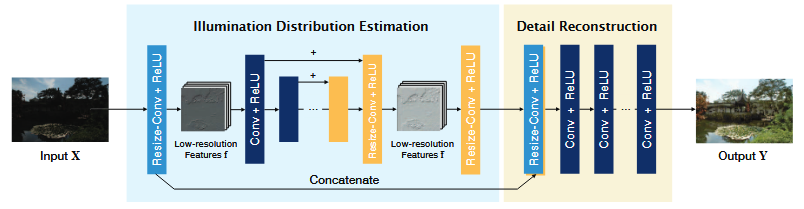
\includegraphics[width=0.8\columnwidth]{GLADNet}
	
	\begin{subfigure}{\textwidth}
		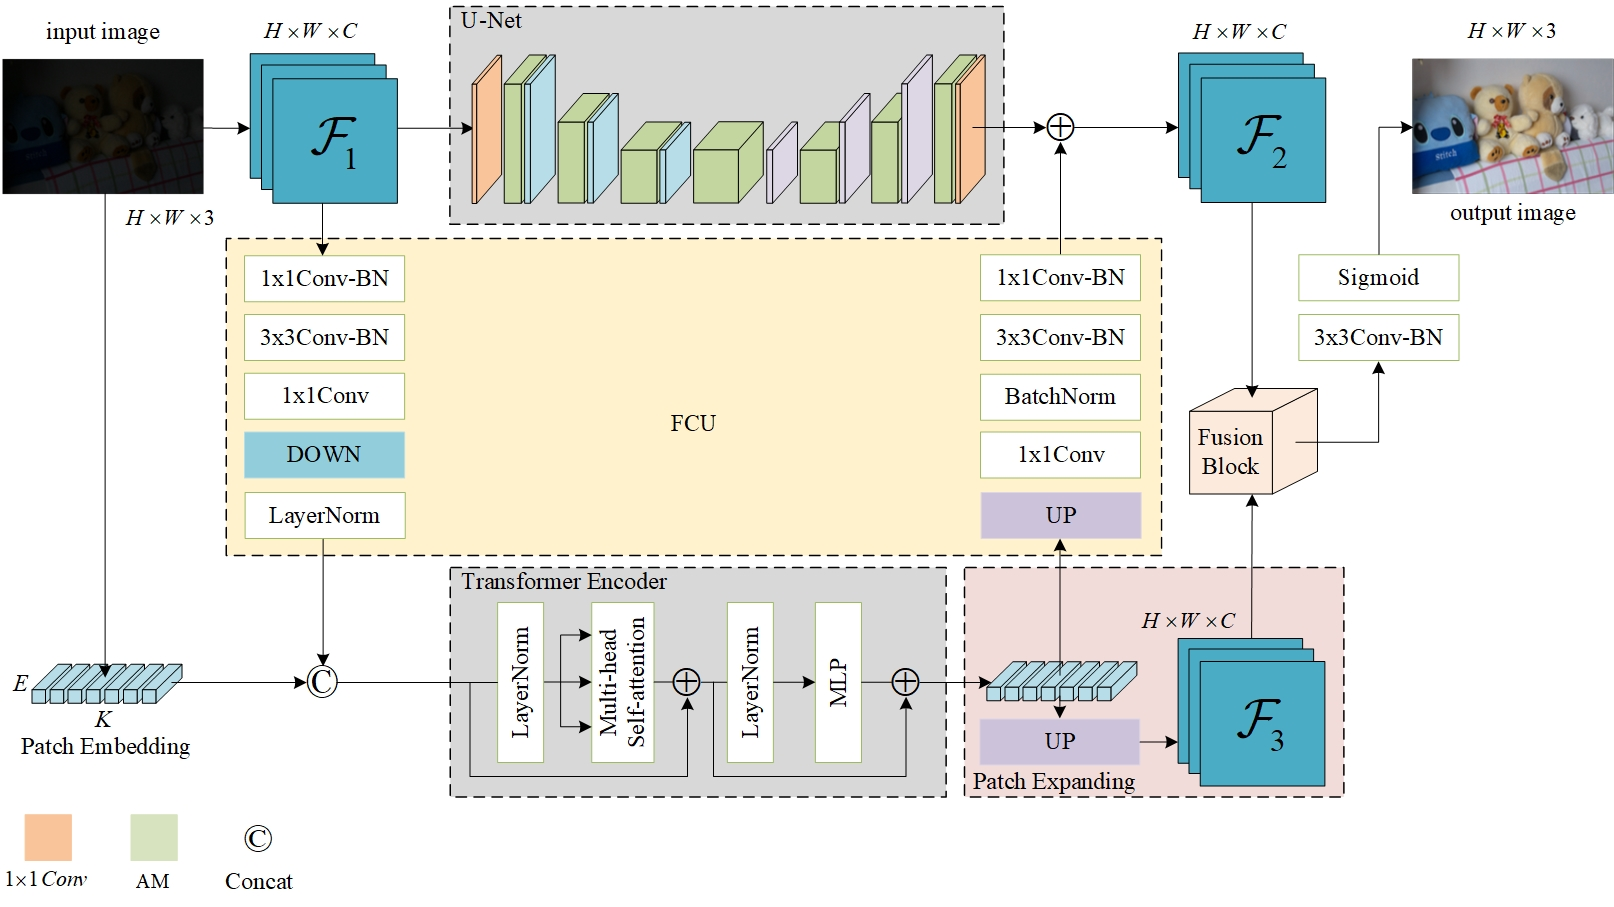
\includegraphics[width=\linewidth]{picture/LLIE/My Architecture/The proposed initial architecture.jpg}
		\captionsetup{font=scriptsize}
		\caption{PACUT}
		\label{fig: First Architecture}
	\end{subfigure}\\
	\begin{subfigure}{0.4\textwidth}
		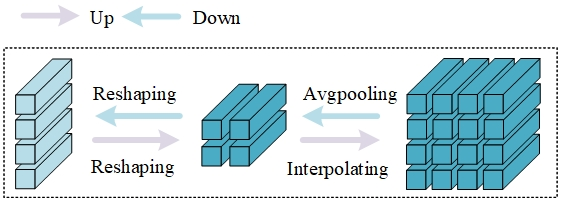
\includegraphics[width=\linewidth]{picture/LLIE/My Architecture/Up-sampling and down-sampling}
		\captionsetup{font=scriptsize}
		\caption{Up-sampling and Down-sampling}
		\label{fig: Up-sampling and down-sampling}
	\end{subfigure} \
	\begin{subfigure}{0.4\textwidth}
		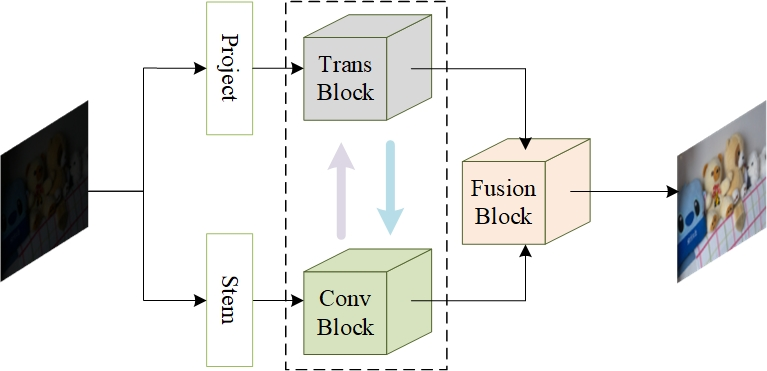
\includegraphics[width=\linewidth]{picture/LLIE/My Architecture/The proposed initial architecture(Abstract Picture)}
		\captionsetup{font=scriptsize}
		\caption{Thumbnail of PACUT}
		\label{fig: The proposed initial architecture(Abstract Picture)}	
	\end{subfigure}
	%\captionsetup{font=scriptsize}
	\caption{
		\label{fig: PACUT}
		PACUT 模型结构。图\ref{fig: First Architecture} CNN 分支和 Transformer 分支以及 FCU (Feature Coupling Unit)。图\ref{fig: Up-sampling and down-sampling} 特征映射和 Patch embeddings 空间对齐的上采样和下采样过程。 图\ref{fig: The proposed initial architecture(Abstract Picture)} PACUT 的缩略图。PACUT 结构受 Conformer\upcite{peng2021conformer}启发,将原来结构中 CNN 分支的 ResNet 结构修改为 U-Net 结构。其采用一个 U-Net 和 ViT 的并行架构,通过 U-Net 结构得到一个弱恢复的弱特征图 $\mathcal{F}_2$,通过 ViT 融合的特征可以初步增强弱特征图 $\mathcal{F}_2$,ViT 的输出经过 Patch Expanding 的特征图 $\mathcal{F}_3$ 经过与 U-Net 输出的特征图 $\mathcal{F}_2$ 融合之后得到一个初步恢复的图片 output image,用以后续参与图片的进一步恢复。
	}
\end{figure}

具体而言,PACUT架构由两个并行分支、一个Stem模块、一个特征连接单元(FCU, Feature Coupling Unit)以及一个为两个分支设计的融合模块(Fusion Block)组成。Stem模块由VGG16网络的前四层构成,截至第一个最大池化层,其主要功能是提取图像的初始局部特征,如边缘和纹理等,随后将这些特征输入到CNN分支。CNN分支采用了改进的U-Net网络结构,而Transformer分支则由一个经过修改的Vision Transformer构成,去除了分类功能,仅保留特征提取功能。

在这种并行结构中,CNN分支和Transformer分支分别专注于最大程度地保留局部特征和全局表征。FCU作为一种桥接模块,其作用是融合CNN分支中的局部特征和Transformer分支中的全局表征,如图\ref{fig: First Architecture} 所示。FCU从第二步开始应用,因为两个分支的初始特征虽相同,但表征形式不同。在整个网络中,FCU通过双向交互融合特征图和Patch Embeddings。

最终,两个分支的特征都被送入特征融合模块进行处理。对于Transformer分支,为了更有效地利用长距离特征,我们在进行Patch Expanding操作之前,通过FCU与CNN分支进行融合。最后,两个分支的输出通过特征融合模块处理后,生成最终的增强图像。在训练过程中,我们采用了结合$\mathcal{L}_1$和SSIM损失函数的策略,以优化模型在像素级误差和感知质量方面的表现。

\subsection{CNN 分支}

在PACUT架构中,CNN分支基于U-Net网络结构,这是一种原本为图像分割任务设计的网络架构,但其在图像增强领域同样展现出卓越的性能。U-Net的显著特点在于其对称的编码器-解码器结构和编码器与解码器之间的跳跃连接。在本研究中,CNN分支的目标是从输入的低光照图像(LLI)中提取丰富的特征,包括边缘、纹理、颜色和亮度信息,并最终生成增强的图像(EI)。


\begin{figure}[htb]
	% read manual to see what [ht] means and for other possible options
	\centering 
	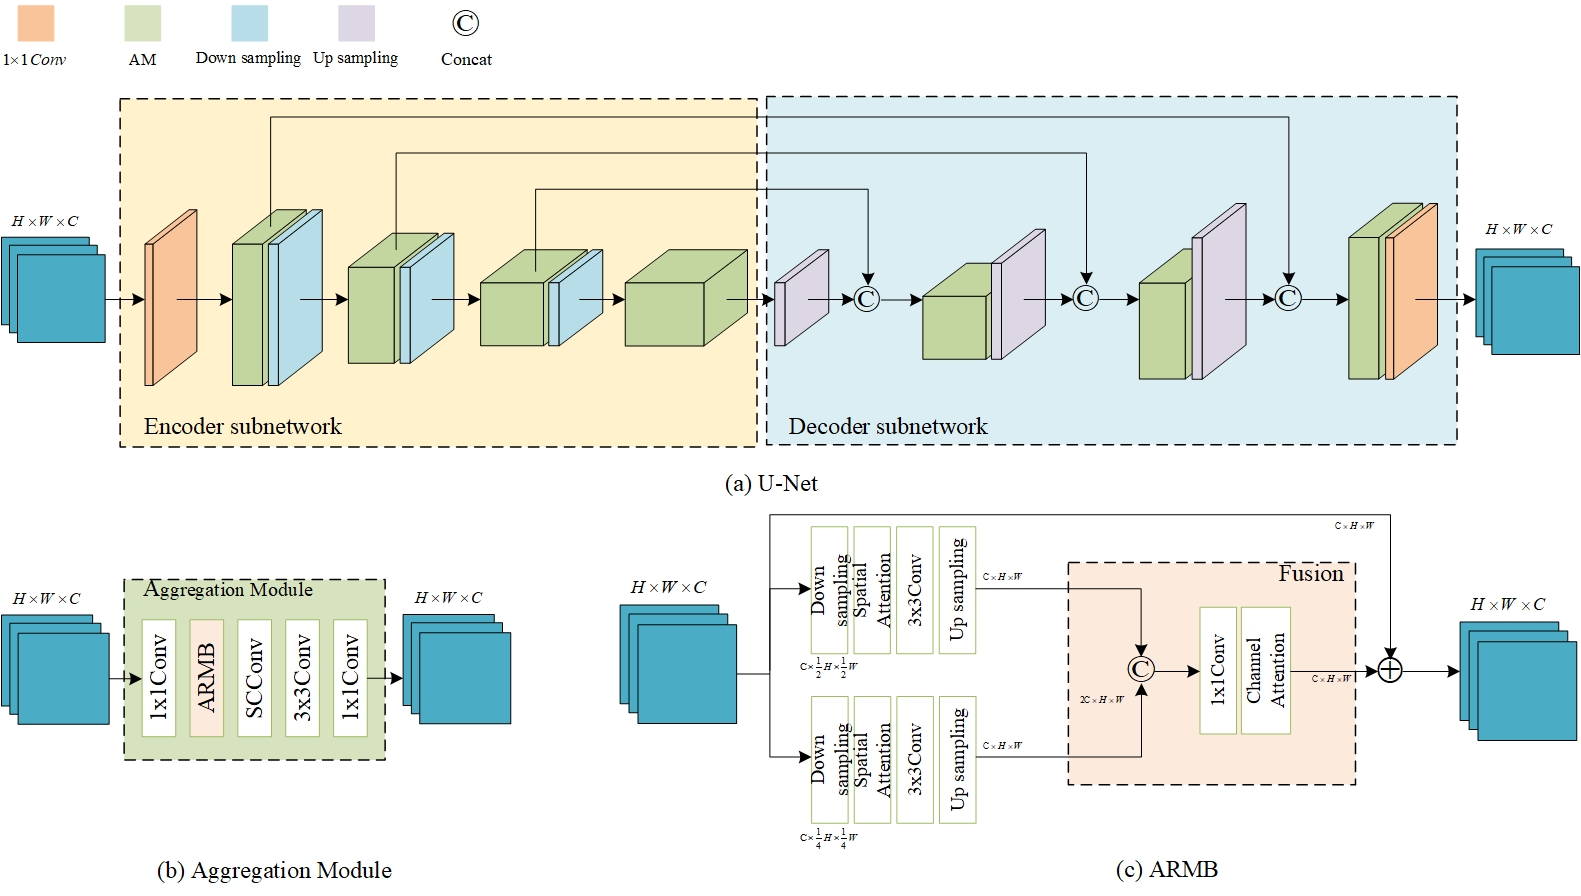
\includegraphics[width=\columnwidth]{picture/LLIE/My Architecture/U-Net and AM}
	%\captionsetup{font=scriptsize}
	\caption{
		\label{fig: U-Net and AM} 
		CNN分支及其所属的模块。
	}
\end{figure}

针对低光照图像增强任务,我们设计了UNetEnhance模型,用于PACUT的CNN分支。该模型在经典U-Net架构的基础上进行了多项改进,以增强其处理低光照环境下图像的能力。这些改进包括更深的网络结构、改进的特征融合机制和高效的信息传递路径。UNetEnhance模型的结构如图\ref{fig: U-Net and AM}所示,它由两部分组成:1) 编码器子网络(Encoder Subnetwork)和2) 解码器子网络(Decoder Subnetwork)。编码器子网络采用了多层卷积网络结构,在每层中集成了空间注意力机制和通道注意力机制\upcite{woo2018cbam}。与传统U-Net相比,这种设计增加了网络的深度,使其能够捕获更丰富的特征信息。解码器部分则采用了上采样和卷积操作,逐步恢复图像的空间分辨率,并引入了改进的特征融合策略,将编码器中的低级特征与解码器的高级特征有效结合,以更好地重建图像细节。此外,UNetEnhance模型在跳跃连接的设计上进行了优化,以更有效地传递编码器中的特征信息到解码器,这些连接不仅帮助保留了在下采样过程中可能丢失的细节信息,还增强了网络的特征重建能力。模型的输出层经过特别设计,以确保输出图像在视觉上的质量和连贯性,我们通过精确调整解码器子网络中的卷积操作,将解码器的输出转换为与原始输入图像相同尺寸的增强图像。
	
假设$I_{LLI}$表示输入的低光照图像,$I_{EI}$表示输出的增强图像。编码器子网络$\mathcal{E}$和解码器子网络$\mathcal{D}$的操作可以表示为:

\begin{equation}
	I_{EI} = \mathcal{D} \left( \mathcal{E} \left( I_{LLI} \right) \right)
\end{equation}

对于AM集成模块(图\ref{fig: U-Net and AM}b),其操作可表示为:

\begin{equation}
	\text{AM}_{i}(x) = f^{1 \times 1} \left(f^{3 \times 3} \left(\text{SCConv}\left( \text{ARMB} \left( f^{1 \times 1} (x)\right)\right)\right)\right)
\end{equation}

其中,$f^{1\times1}$为$1 \times 1$卷积层,ARMB和SCConv的操作依据其内部结构进行。

编码器首先通过一个$1 \times 1$卷积层处理输入图像,用于提取初始特征。然后连续通过四个单元,前三个单元每一个都由一个AM集成模块$\text{AM}_i$和一个池化层组成,第四个单元仅包含一个AM集成模块。AM集成模块由一系列卷积层和特殊的注意力机制组成的复杂结构,包括ARMB模块和SCConv模块。

解码器首先通过一个上采样模块,然后与$\text{AM}_{3}$进行拼接操作,接着通过$\text{AM}_{5}$集成模块和上采样模块,再与$\text{AM}_{2}$拼接,然后通过$\text{AM}_{6}$集成模块和上采样模块,最后与$\text{AM}_{1}$拼接,最终通过$\text{AM}_{7}$集成模块和$1 \times 1$卷积层。

\subsubsection{注意力残差多尺度块}

注意力残差多尺度块(ARMB, Attention Residual Merging Block) 是一种用于深度学习模型中的结构单元,特别是在处理图像相关任务时,它的主要作用是融合来自不同来源的特征,并通过注意力机制增强模型对关键信息的关注。其核心作用之一是融合来自模型不同层或不同分支的特征。这种融合有助于结合低级特征(如边缘和纹理)和高级特征(如对象部分和语义信息),从而提升模型的表现力。ARMB 中的注意力机制有助于 UNetEnhance 更加关注于图像中的重要区域或特征。通过加权重要特征,ARMB 可以提高模型对关键信息的敏感性。ARMB 通过残差连接来解决深度神经网络中的梯度消失问题。如图\ref{fig: U-Net and AM}c 所示,残差连接允许信息直接从早期层传递到后续层,从而保持信息流的连续性。

模块对输入特征 $\mathcal{F}$ 进行两次分支下采样,分别获取尺寸为 $\dfrac{1}{2}$ 和 $\dfrac{1}{4}$ 的特征。每个分支使用空间注意力 (Spatial Attention) 过滤噪声,通过 $3 \times 3$ 卷积层提取特征,并通过上采样恢复到原始尺寸。将两个特征图拼接后,通过$ 1 \times 1$ 卷积层处理,再应用通道注意力 (Channel Attention) 进行特征加权,最后通过跳跃连接与原始输 $\mathcal{F}$ 合并,得到最终特征图。

假设 $\mathcal{F}_{in}$ 是输入特征图,$\mathcal{F}_{out}$ 是输出特征图,$\mathcal{F}_{i}^\prime$ 表示对特征图进行裁剪或放大,见下式:

\begin{equation}
	\begin{aligned}
		&\mathcal{F}^\prime_{\frac{1}{2}} = \text{Resize}\left(\mathcal{F}_{in},\left(\frac{H}{2},\frac{W}{2}\right)\right), \\
		&\mathcal{F}^\prime_{\frac{1}{4}} = \text{Resize}\left(\mathcal{F}_{in},\left(\frac{H}{4},\frac{W}{4}\right)\right), \\
		&\mathcal{F}_{out} = W_1\mathcal{F}_{out} + W_2\mathcal{C} \left( f^{1 \times 1}  \left[\mathcal{F}^\prime_2 (f^{3 \times 3}(\mathcal{S}(\mathcal{F}^\prime_{\frac{1}{2}}))), \mathcal{F}^\prime_4 (f^{3 \times 3}(\mathcal{S}(\mathcal{F}^\prime_{\frac{1}{4}})))\right] \right).
	\end{aligned}
	\label{eq: ARMB}
\end{equation}

其中 $\mathcal{S}$ 和 $\mathcal{C}$ 分别表示空间注意力函数和通道注意力函数,$W_1$ 和 $W_2$ 为对应的特征图权重。

在ARMB模块内部,我们引入了SCConv模块,这是一种专门设计用于特征冗余的空间和通道重构卷积。SCConv模块由两个关键子模块组成:空间重构单元(SRU)和通道重构单元(CRU)。SRU的主要作用是通过门控机制对特征进行选择性激活,从而增强模型对于关键特征的关注度。具体来说,SRU通过学习特征的空间分布,实现对特征图中重要区域的强调和非重要区域的抑制。这种机制使得模型能够更加有效地处理图像中的空间信息,提高特征提取的精确性。

另一方面,CRU负责特征的融合和重构。它通过分析和整合不同通道上的特征信息,优化特征表示的通道维度。CRU的设计基于这样一个假设:不同通道的特征具有不同的重要性和贡献度。因此,CRU通过学习不同通道间的关系,实现对特征的有效融合,从而提高了特征表示的丰富性和鲁棒性。这一过程不仅增强了模型对于通道信息的利用效率,还提升了整体网络对于复杂图像内容的理解能力。

综上所述,SCConv模块通过SRU和CRU的协同作用,实现了对特征的空间和通道维度的有效重构,从而优化了特征表示的质量和效率。这种设计在处理图像特征时,不仅提高了特征提取的精度,还增强了模型对于复杂图像内容的处理能力。
	
\subsection{Transformer分支}
	
Transformer分支的核心是基于视觉变换器(ViT, Vision Transformer)架构,其主要职责在于从输入图像中提炼出全局特征。这一分支专注于揭示图像中的长距离依赖关系,其目的是为CNN分支提供的局部特征提取过程提供补充和增强。ViT架构通过将图像划分为一系列小块(patches),并将这些块转换为一维序列,从而使得模型能够利用自注意力机制来捕获这些块之间的复杂关系。
	
\subsubsection{嵌入块}
	
在深度学习和计算机视觉领域,嵌入块(Patch Embedding)是一种关键操作,它涉及将图像划分为较小的单元(称为patches),随后将这些单元转换为一系列向量,这些向量随后作为模型的输入。此过程的核心在于将图像的空间特征转换为可以被深度学习模型处理的形式。
	
\begin{figure}[htb]
	% read manual to see what [ht] means and for other possible options
	\centering 
	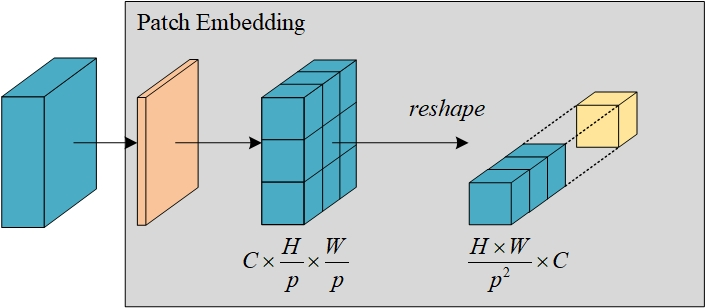
\includegraphics[width=0.5\columnwidth]{picture/LLIE/My Architecture/Patch Embedding}
	%\captionsetup{font=scriptsize}
	\caption{
		\label{fig: Patch Embedding} 
		嵌入块的一般性过程。
	}
\end{figure}
	
具体来说,对于原始的低光照图像 $P_1$,首先执行尺寸压缩操作,以适配预训练的视觉变换器(Vision Transformer, ViT)模型的权重。此操作将低光照图像(LLI)转换为一系列的Patch Embeddings,生成576个 D 维的特征向量,其中每个向量对应于一个$16 \times 16$的图像块(patch)。接下来,将$384 \times 384$的特征向量重排列为576个$16\times16$的图像块,每个图像块随后被展平(flatten)为256维的向量。考虑到图像的三通道特性,实际上每个通道被展平为256维,从而形成总计$256 \times 3$维的向量$\ell_1$。

此过程的关键在于将二维图像数据转换为一维向量序列,这为后续的Transformer模型处理提供了适合的输入格式。通过这种方式,模型能够有效地处理图像数据,捕获重要的空间和颜色特征,从而为深度学习任务提供强大的数据基础。
	
\begin{figure}[htb]
	% read manual to see what [ht] means and for other possible options
	\centering 
	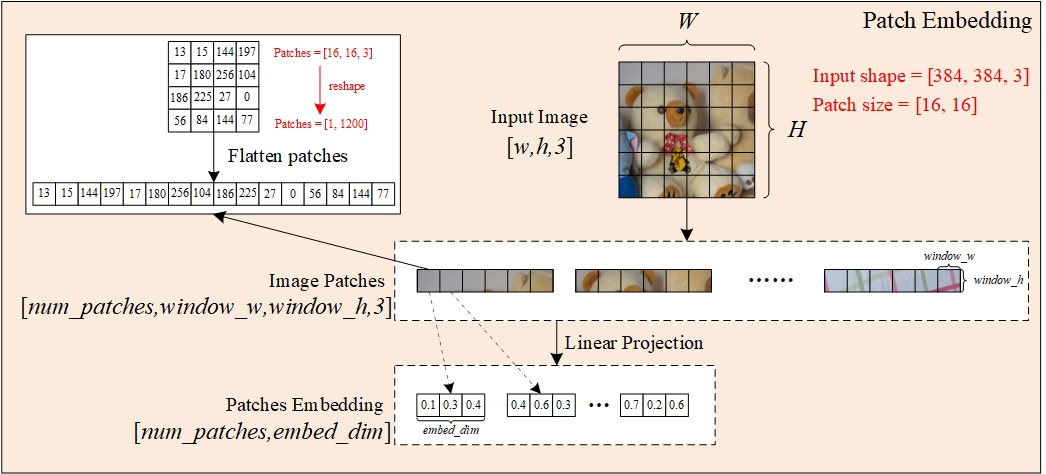
\includegraphics[width=0.8\columnwidth]{picture/LLIE/My Architecture/Patch Embedding(ViT)}
	%\captionsetup{font=scriptsize}
	\caption{
		\label{fig: Patch Embedding(ViT)} 
		Transformer 分支中嵌入块的过程。
	}
\end{figure}
	
为了进一步处理这些向量,我们采用一个线性投影(Linear Projection)操作,将$\ell_1$转换为D维的向量。这一转换过程不仅保留了原始图像块的关键信息,而且使其适配于深度学习模型的输入要求。如图\ref{fig: Patch Embedding(ViT)}所示,这一过程是将图像的空间特征转换为模型可以有效处理的形式的关键步骤。通过这种方式,模型能够更有效地处理和理解图像内容,从而在低光照图像增强任务中实现更优的性能。
	
嵌入块的具体过程可以被描述为下列过程:
	
\begin{itemize}
	\item[$\bullet$] 
	输入图像 $X \in \mathbb{R}^{H \times W \times C}$,其中 $H$,$W$和$C$ 分别代表图像的高度、宽度和通道数。
	\item[$\bullet$]
	图像被分割成 $N$ 个大小为 $P \times P$ 的块,每个块被展平并线性投影到 D 维空间,得到嵌入块 $E \in \mathbb{R}^{N \times D}$
\end{itemize}

图\ref{fig: First Architecture} 展示了在 Patch Embedding 过程之后,特征 $\mathcal{F}_1$ 经过必要的变换处理,以便与向量 $\ell_1$ 进行拼接操作。这一步骤是必要的,因为未经处理的特征 $\mathcal{F}_1$ 无法直接与向量 $\ell_1$ 进行有效的拼接。

在本研究中,我们采用了 $20 \times 20$ 的 Patch 尺寸进行 Embedding。然而,选择此尺寸的适宜性依赖于输入图像的尺寸及其包含的细节的重要性。对于那些含有微小但关键特征的图像,较小的 Patch 尺寸可能更为适宜,因为它们能够更精确地捕捉这些细节。相反,较大的 Patch 尺寸可能更适合于捕获图像中的高层次抽象特征。因此,为了在细节捕捉和高层次特征表示之间找到最佳平衡点,我们的后续工作将包括对不同 Patch 尺寸的实验性探索,以确保模型能够有效地处理和理解图像中的关键信息。
	
\subsubsection{位置编码}
	
在Transformer中,由于缺乏像卷积神经网络 (CNN) 那样的固有空间结构,需要一种方法来告知模型不同块之间的相对或绝对位置。位置编码就是为了解决这个问题而设计的。
	
位置编码通常是通过将一个固定的或可学习的编码添加到每个块的 embedding 中来实现的。这个编码是根据块在原始图像中的位置计算得出的。一种常见的方法是使用正弦和余弦函数的组合来生成每个位置的编码。例如,对于位置 pos 和维度 i,编码可以被表示为式\ref{eq: positional encoding}
	
\begin{equation}
	\begin{aligned}
		&\text{PE}(\text{pos}, \ 2i) = \sin \left(\frac{\text{pos}}{10000^{\frac{2i}{D}}}\right) \\
		&\text{PE}(\text{pos}, \ 2i + 1) = \cos \left(\frac{\text{pos}}{10000^{\frac{2i}{D}}}\right)
	\end{aligned}
	\label{eq: positional encoding}
\end{equation}
	
其中,D 是 embedding 的维度。计算出的 Positional Encoding 被加到每个 patch 的 embedding 上。位置编码为 $PE \in \mathbb{R}^{N \times D}$,Positional Encoding 被描述为 $E_{pos} = E + PE$。 这样,即使在多头自注意力机制中,模型也能够利用这些编码来理解和利用 patches 之间的相对位置信息。在ViT中,Positional Encoding对于模型理解图像内容至关重要。它允许模型捕捉到图像中的空间层次结构和对象之间的相对位置关系,这对于图像理解任务来说是非常重要的。
	
我们采用 timm 库来创建预训练的ViT模型,并移除了原始的分类头,在 timm 库中创建的预训练 ViT 模型已经内置了Positional Encoding的过程。
	
\subsubsection{Transformer编码器}
	
在视觉变换器 (ViT) 架构中,Transformer Encoder 是核心组件,负责处理图像的序列化表示。经过位置编码的 Patch Embeddings 被送入 Transformer 的编码器。如图\ref{fig: First Architecture} 所示,Transformer 编码器主要设计两个主要步骤,包括多头自注意力机制 (Multi-head Self-Attention) 和多层感知器 (Multi-Layer Perceptron)。这些组件共同工作,以捕获图像中的复杂特征和长距离依赖关系。
	
其中,多头自注意力机制允许模型在处理每个图像块时同时考虑其他所有块的信息。通过这种方式,模型能够捕获图像中不同区域之间的复杂关系和依赖性。在多头自注意力中,注意力机制被分割成多个“头”,每个头学习图像的不同方面,从而提高了模型的表达能力。MLP 由多个线性层和非线性激活函数组成,它为模型引入了必要的非线性处理能力。这种非线性是处理复杂数据(如图像)时不可或缺的,因为它允许模型学习更加复杂和抽象的特征表示。
	
对于每个 Transformer 层 $l$,输入 $X_l$ 经过以下过程:
	
\begin{itemize}
	\item[1)] 
	多头自注意力 (MSA):
	\begin{equation}
		\begin{aligned}
			\text{MSA}(X_l) = [\text{head}_1, \text{head}_2, \ldots, \text{head}_k] W^{O}
		\end{aligned}
		\label{eq: MSA}
	\end{equation}
	其中每个头(head)是 $\text{head}_i = \text{Attention}\left(X_l W_i^Q, X_l W_i^K, X_l W_i^V \right)$。Attention 机制通常定义为
	\begin{equation}
		\begin{aligned}
			\text{Attention}(Q, K, V) = \text{softmax} \left(\frac{QK^T}{\sqrt{d_k}} \right) V
		\end{aligned}
		\label{eq: Attention}
	\end{equation}
	其中 $d_k$ 是 key 向量的维度。
		
	\item[2)]
	残差连接和层归一化:
	\begin{equation}
		\begin{aligned}
			X_l^\prime = \text{LayerNorm} \left(X_l + \text{MSA}(X_l)\right)
		\end{aligned}
		\label{eq: Residual Connection}
	\end{equation}
	
	\item[3)]
	多层感知机:
	MLP 包含两个全连接层和一个激活函数,即 $\text{MLP} (X_l^\prime) = \text{FC}\left(\text{GELU}\left(\text{FC}(X_l^\prime)\right)\right)$
		
	\item[4)]
	第二个残差连接和层归一化:
	\begin{equation}
		\begin{aligned}
			\displaystyle X_{l+1} = \text{LayerNorm} (X_l^\prime + \text{MLP}(X_l^\prime))
		\end{aligned}
		\label{eq: layernorm}
	\end{equation}
\end{itemize}
	
经过一层 Transformer编码器处理后,得到的输出 $X_L$ 可以用于下一步的处理。
	
Transformer编码器通过多层自注意力和 MLP 的堆叠,有效地处理图像数据,捕获长距离依赖关系,并学习复杂的特征表示。这种架构使得模型能够处理高维度的图像数据,并提取有用的特征,为后续的图像处理任务提供强大的特征支持。
	
\subsubsection{特征耦合单元}

在 PACUT 架构中,CNN 分支产生的特征映射与 Transformer 分支的 Patch Embedding 之间的有效融合是一个关键挑战。为了解决这一问题,我们引入了特征耦合单元(FCU),它通过交互式方法将局部特征与全局表示进行连续耦合,从而消除两者之间的不一致性。

首先,我们认识到 CNN 分支和 Transformer 分支之间特征维度的不一致性。CNN 分支的特征图维度为$H \times W \times C$,其中$H$, $W$和$C$分别代表高度、宽度和通道数。而 Transformer 分支的嵌入块形状为$K \times D$,其中 $K$ 和 $D$ 分别表示图像块的数量和嵌入的维度。在用于分类的视觉变换器模型中,嵌入块的形状为$\left(K+1 \right) \times D$,其中额外的 1 代表类别嵌入(Class Token)。然而,在我们的 Transformer 分支中,我们去除了类别嵌入,以便更好地适应非分类任务。

类别嵌入是一种特殊的嵌入,用于代表整个输入序列的全局信息。虽然这在图像分类任务中至关重要,但在图像增强等非分类任务中,其重要性相对较低。因此,去除类别嵌入不会显著影响特征图的恢复能力。

为了实现 CNN 特征图和 Transformer Patch Embedding 之间的融合,我们首先通过$1 \times 1$卷积调整 CNN 特征图的通道维度,以匹配 Patch Embedding 的维度。接着,使用下采样模块(如图\ref{fig: Up-sampling and down-sampling} 所示)调整空间尺寸。完成这些步骤后,特征图与 Patch Embedding 进行融合(如图\ref{fig: First Architecture} 所示)。当特征从 Transformer 分支传输到 CNN 分支时,我们采用上采样(如图 \ref{fig: Up-sampling and down-sampling} 所示)来调整空间比例,并通过$ 1 \times 1$卷积调整通道尺寸,以便与 CNN 特征图对齐。此外,LayerNorm 和 BatchNorm 被用于特征的正则化。

最后,考虑到特征映射和嵌入块之间存在的语义差异——前者源自局部卷积操作,后者则通过自注意力机制聚合——FCU 的应用至关重要,以填补这一语义鸿沟,确保两种特征的有效融合。
	
\subsubsection{特征融合模块}
	
\begin{figure}[htb]
	% read manual to see what [ht] means and for other possible options
	\centering 
	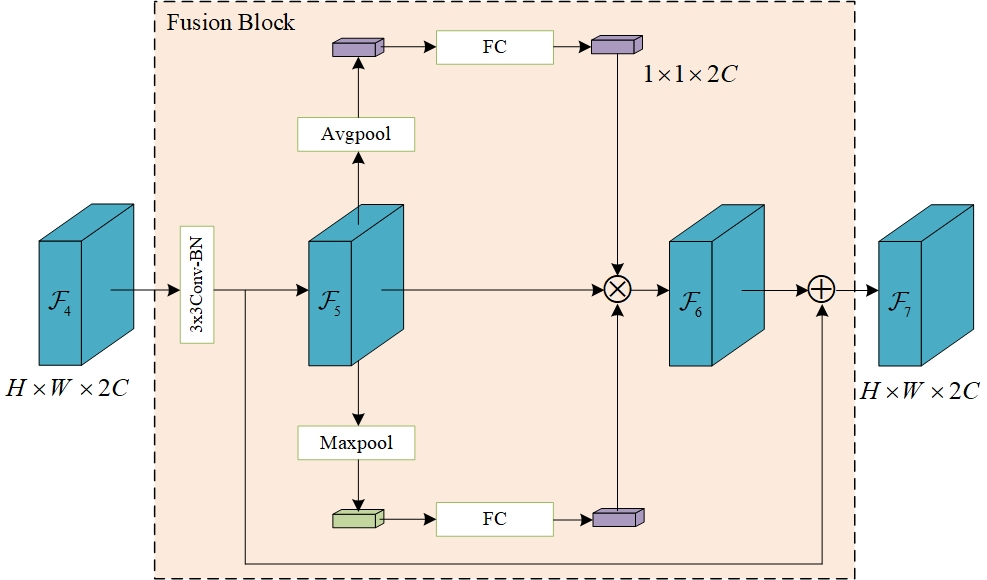
\includegraphics[width=0.7\columnwidth]{picture/LLIE/My Architecture/Fusion Block}
	%\captionsetup{font=scriptsize}
	\caption{
		\label{fig: Fusion Block} 
		融合模块的结构。
	}
\end{figure}
	
在U型网络编码器结构中,浅层特征包含丰富的纹理信息和颜色信息,多层卷积得到的高层特征包含全局信息。对于弱光图像增强,需要尽可能的保留输出结果中的颜色信息。为此,PACUT 结构引入了图像通道来保留具由特定颜色特征的信息,从而更好的恢复暗区信息,防止亮区信息过度曝光。具体来说,在U型网络中设计了三个条约链接,将浅层特征发送到后头,以解决颜色信息丢失的问题。为了有效的融合视觉变换器和U型特征,提出一个如图\ref{fig: Fusion Block}所示的特征融合模块。其输入由两部分组成,即 PACUT 中CNN分支得到的特征 $\mathcal{F}_2$ 和Transformer分支中块展开(Patch Expanding)后得到的特征 $\mathcal{F}_3$。该模块包含两个步骤。
	
第一步,将两个尺寸为 $H \times W \times C$的特征图连接起来,形成一个尺寸为 $H \times W \times 2C$的特征图 $\mathcal{F}_4$。以该特征图为输入,通过 $3 \times 3$ 的卷积核,步长为1,进一步得到大小为 $H \times W \times 2C$ 的特征图 $\mathcal{F}_5$。这个过程可以有效的捕获颜色信息,表示为 
	
\begin{equation}
	\begin{aligned}
		\mathcal{F}_5 = \delta \left( f^{3 \times 3} (\mathcal{F}_4)\right)
	\end{aligned}
	\label{eq: capture color information}
\end{equation}
	
在第二步中,通过为不同的通道分配适当的权重来重新校准特征映射 $\mathcal{F}_5$。为此,构建一个由两个加权支路和一个短连接组成的模块,如 Fig. \ref{fig: Fusion Block}所示。首先,通过全局平均池化将特征映射 $\mathcal{F}_5$ 压缩成 $1 \times 1 \times 2C$ 个向量;同时,特征映射 $\mathcal{F}_5$ 还需要进行全局最大池化,以尽可能的保留纹理细节。得到的 $1 \times 1 \times 2C$ 向量中的每一个元素表示通道信息。它们的公式为
	
\begin{equation}
	\begin{aligned}
		\mathcal{Z}_{GAP} = \frac{1}{H \times W} \sum_{i}^{H} \sum_{j}^{W} {\mathcal{F}_5}_C (i,j)
	\end{aligned}
	\label{eq: avgpool}
\end{equation}
	
\begin{equation}
	\begin{aligned}
		\mathcal{Z}_{GMP} = \max \left( \mathcal{F}_5 \right)
	\end{aligned}
	\label{eq: maxpool}
\end{equation}
	
其中 $\mathcal{Z}_{GAP}$ 和 $\mathcal{Z}_{GMP}$ 分别为全局平均池化和全局最大池化得到的特征值,${\mathcal{F}_5}_C$ 为 $\mathcal{F}_5$ 的第 $C$ 个通道的特征。接下来,这两个压缩向量通过两个完全连接的层进行加权,以获得各自的权重向量。最后,通过特征向量乘以相应的权值,得到一个重新校准后,大小为 $H \times W \times 2C$ 的特征图 $\mathcal{F}_7$
	
\begin{equation}
	\begin{aligned}
		\mathcal{F}_7 = \sigma \left( W_2 \delta (W_1 Z_{GAP}) \right) \cdot M \cdot \sigma \left( W_2 \delta (W_1 Z_{GMP})\right) +  \mathcal{F}_5
	\end{aligned}
	\label{eq: recalibrated feature map}
\end{equation}
	
其中 $W_1$ 和 $W_2$ 是两个完全连接层的权值。

\subsection{损失函数}

在本研究中,为了优化图像重建和内容生成的质量,我们提出了一个综合的联合损失函数,用于指导模型生成高质量的增强图像。该联合损失函数综合考虑了多个关键因素,以确保生成图像的质量和真实性。具体地,联合损失函数定义为:

\begin{equation}
	\begin{aligned}
		\mathcal{L}_{all} = w_0 \mathcal{L}_{hub} + w_1 \mathcal{L}_{per} + w_2 \mathcal{L}_{\text{SSIM}}
	\end{aligned}
	\label{eq: loss function}
\end{equation}

其中,$\mathcal{L}_{hub}$ 代表休伯(Huber)损失\upcite{huber1992robust},$\mathcal{L}_{per}$代表感知损失\upcite{johnson2016perceptual},而$\mathcal{L}_{\text{SSIM}}$代表结构相似性(SSIM)损失\upcite{wang2004image}。这些损失函数的组合旨在平衡图像的像素级精度和感知质量。

Huber 损失($\mathcal{L}_{hub}$)是一种结合了均方误差和绝对误差的损失函数,用于减少对异常值的敏感性,从而提高模型的鲁棒性。感知损失($\mathcal{L}_{per}$)则关注于图像的高级特征和内容,通过比较深层网络中的特征表示来评估图像之间的感知差异。结构相似性指数(SSIM)损失($\mathcal{L}_{\text{SSIM}}$)则用于评估图像的结构、亮度和对比度等方面的相似性,以确保生成图像在视觉上与原始图像保持一致性。

权重$w_0$, $w_1$和$w_2$分别对应于这三种损失的相对重要性,通过实验调整以达到最佳的图像增强效果。通过这种方式,联合损失函数能够有效地平衡像素级精度和感知质量,从而生成在视觉上更加令人满意的增强图像。

我们设$w_0 = 1$, $w_1 = 0.006$和$w_2 = 0.01$。

通过最小化PACUT的输出与正常照明图像之间的误差,利用休伯损失指导PACUT生成结构完整的增强图像。令$I_{GT}$为真实图像,$I_{EI}$为增强图像。休伯损失可以表示为式\ref{eq: huber loss}

\begin{equation}
	\mathcal{L}_{hub}(\delta)= \frac{1}{N}\sum_{i=1}^{N}
	\left\{
	\begin{aligned}
		&\displaystyle{\frac{1}{2}{\left\|I_{\text{GT}} - I_{\text{EI}} \right\|}_2^{2}, \left\| I_{GT} -I_{EI} \right\| < \delta }, \\
		&\delta\left({\left\|I_{\text{GT}} - I_{\text{EI}} \right\|}_1 - \frac{1}{2}\delta \right), \left\| I_{\text{GT}} -I_{\text{EI}} \right\| \geq \delta.
	\end{aligned}
	\label{eq: huber loss}
	\right.
\end{equation}

$\mathcal{L}_2$-loss但容易受离群点的影响,$\mathcal{L}_1$-loss对离群点更加健壮但是收敛慢,Huber Loss 则是一种将MSE与MAE结合起来,取两者优点的损失函数,也被称作Smooth Mean Absolute Error Loss。其原理很简单,就是在误差接近0时使用$\mathcal{L}_2$-loss,误差较大时使用$\mathcal{L}_1$-loss

然而,休伯损失容易同时平滑增强图像的噪点和细节。为了保留图像的纹理信息,提高图像内容质量,我们引入感知损失,用于比较图像之间的高层次差异,感知损失可以表示为式\ref{eq: perceptual loss}。

\begin{equation}
	\begin{aligned}
		\mathcal{L}_{feat}^{\phi,j} (I_{GT},I_{EI}) = \frac{1}{C_{j}H_{j}W_{j}}{\left\| \phi_{j}(I_{GT})-\phi_{j}(I_{EI})\right\|}_{2}^2
	\end{aligned}
	\label{eq: perceptual loss}
\end{equation}

其中$I_{GT}$为输出图像,$I_{EI}$为目标图像,$\phi$为损失网络。$\phi_{j}(x)$为处理图像$x$时损失网络$\phi$的第$j$层的激活情况,如果$j$是一个卷积层,那么$\phi_{j}(x)$将是形状$C_{j} \times H_{j} \times W_{j}$的特征映射,特征重建损失是特征表示之间的欧式距离。

此外,为了使得恢复图像的亮度、对比度和结构与真实图像更加接近和同时细化恢复图像的细节,我们引入了结构相似性损失,结构相似性损失可以表示为式

每个像素$p$的\text{SSIM}被定义为式\ref{eq: revised_SSIM loss}

\begin{equation}
	\begin{aligned}
		\text{SSIM}(p) &= \frac{2\mu_{x}\mu_{y}+C_{1}}{\mu_{x}^2+\mu_{y}^2+C_{1}} \cdot \frac{2\sigma_{xy}+C_{2}}{\sigma_{x}^2+\sigma_{y}^{2}+C_{2}} \\
		&= l(p)\cdot cs(p)
	\end{aligned}
	\label{eq: SSIM}
\end{equation}

其中省略了均值和标准偏差对像素$p$的依赖性,均值和标准差是用标准偏差为$\sigma_G,G_{\sigma_G}$

\begin{equation}
	\begin{aligned}
		&\varepsilon(p)=1-\text{SSIM}(p): \\  &\mathcal{L}^{\text{SSIM}}(P)=\frac{1}{N}\sum_{p \in P}1-\text{SSIM}(p).
	\end{aligned}
	\label{eq: SSIM loss}
\end{equation}

eq. \ref{eq: SSIM}表明$\text{SSIM}(p)$需要关注像素$p$的邻域,这个领域的大小取决于$G_{\sigma_G}$,网络的卷积性质允许我们将SSIM损失写为

\begin{equation}
	\begin{aligned}
		\mathcal{L}^{\text{SSIM}}(P)=1-\text{SSIM}(\tilde{p}).
	\end{aligned}
	\label{eq: revised_SSIM loss}
\end{equation}

其中$\tilde{p}$是$P$的中心像素。

\section{实验结果}

在本章节中,我们详细阐述了实验设计,以验证所提出方法的有效性。首先,介绍了实验的具体实施细节,包括网络的实现、所采用的数据集以及评估指标的选择。接着,通过与当前领先技术的比较分析,展示了我们网络在低光图像增强任务中的性能优势。最后,为了深入理解各个网络组件的贡献,我们执行了一系列消融研究,探讨了这些组件在低光图像增强任务中的作用和重要性。

具体来说,实验设置部分详细描述了网络的配置、训练过程中的参数设置、以及用于训练和测试的数据集特性。此外,本研究采用的评估指标被精心选取,以全面反映图像增强的效果,包括定量指标和定性分析。

在性能比较部分,我们的方法与当前最先进的低光图像增强技术进行了对比。这一比较不仅基于传统的性能指标,如图像质量评分,还包括了对增强效果的视觉评估,以展示我们方法的综合优势。

最后,消融实验部分旨在揭示网络各个组成部分的相对重要性和功能。通过系统地移除或修改网络的特定部分,我们能够评估每个组件对最终增强效果的贡献,从而深入理解整个网络的工作机制。这些实验结果为我们的网络设计提供了进一步的洞察和验证。

\subsection{实验设置}

在实验实施方面,PACUT模型是基于Pytorch框架进行实现的。为了确定Transformer分支的最优输入图像尺寸,我们分别设置了384x384和224x224两种分辨率,并通过一系列实验来确定最佳的预训练图像尺寸。在模型训练过程中,我们采用了Adam优化器,其权重衰减系数设定为0.00001,以减少过拟合的风险。此外,模型中所有层的学习率统一设置为0.0001,以确保训练过程的稳定性和收敛性。

基于硬件资源和内存限制的考虑,我们将训练的批处理大小设定为8。同时,为了充分训练模型并确保其泛化能力,我们将训练的epoch数设置为200。所有的实验均在配备 NVIDIA GeForce RTX 4090 显卡的计算平台上进行,以确保训练和测试过程的高效性和可靠性。

\subsection{数据集和评价指标}

为了全面评估我们所提出网络的性能,我们对两个公共数据集(LOL\upcite{wei2018deep}和SCIE\upcite{cai2018learning})进行了实验评估。在评估过程中,我们使用了峰值信噪比(PSNR)\upcite{wang2004image}、结构相似度(SSIM)\upcite{wang2004image}以及自然图像质量评估器(NIQE)\upcite{mittal2012making}等度量指标,以全面衡量图像增强结果的质量。这些评价指标旨在提供对重建图像质量的客观评估,从而深入了解我们提出的网络在低光照环境下的性能表现。

\subsection{对比试验}

我们将所提算法的结果与多个公开可获得的代码进行比较,包括HE\upcite{pisano1998contrast}、LightenNet\upcite{li2018lightennet}、LLNet\upcite{lore2017llnet}、Retinex-Net\upcite{wei2018deep}、MBLLEN\upcite{lv2018mbllen}、EnlightenGAN\upcite{jiang2021enlightengan}、Zero-DCE\upcite{guo2020zero}以及KinD\upcite{zhang2019kindling}。

\begin{table}[!htbp]
	\centering
	\tiny
	\resizebox{\textwidth}{!}{ %按照宽度调整调整表格大小
		\begin{tabular}{>{\centering\arraybackslash}m{2.5cm}|c|c|c|c|c|c}
			
			\hline %添加表格头部粗线
			
			\multirowcell{2}{\textbf{Method}} & \multicolumn{3}{c|}{\makecell{\textbf{LOL}\upcite{wei2018deep}}} & \multicolumn{3}{c}{\makecell{\textbf{SCIE}\upcite{cai2018learning}}} \\
			
			\cline{2-7}
			
			
			      & \textbf{PSNR↑} & \textbf{SSIM↑} & \textbf{NIQE↓} & \textbf{PSNR↑}  & \textbf{SSIM↑} & \textbf{NIQE↓} \\
			
			\hline
			
			input & 7.773 & 0.181 & 0.560 & 17.824 & 0.779 & 0.148  \\
			
			\hline	
			
			HE\upcite{pisano1998contrast}             & 15.467 & 0.504 & 9.531 & 15.342 & 0.741 & 9.232 \\
			LightenNet\upcite{li2018lightennet}       & 10.301 & 0.361 & 7.422 & 13.579 & 0.744 & 8.166 \\
			LLNet\upcite{lore2017llnet}               & \textcolor{blue}{17.953} & 0.704 & \textcolor{red}{3.974} & 12.177 & 0.645 & 4.292 \\
			Retinex-Net\upcite{wei2018deep}           & 16.774 & 0.462 & 5.474 & 12.310 & 0.671 & 7.239 \\ 
			KinD\upcite{zhang2019kindling} 	          & 16.648 & \textcolor{blue}{0.779} & 6.175 & 21.103 & \textcolor{red}{0.838} & 4.195 \\
			MBLLEN\upcite{lv2018mbllen}               & 17.902 & 0.715 & \textcolor{blue}{4.247} & 13.638 & 0.632 & \textcolor{blue}{2.108} \\
			EnlightenGAN\upcite{jiang2021enlightengan}& 17.483 & 0.658 & 4.889 & 18.726 & 0.822 & 5.216 \\
			Zero-DCE\upcite{guo2020zero}              & 17.622 & 0.556 & 7.972 & \textcolor{red}{22.682} & 0.810 & \textcolor{red}{1.158} \\
			\textbf{Ours}                             & \textcolor{red}{22.780} & \textcolor{red}{0.823} & 4.473 & \textcolor{blue}{21.543} & \textcolor{blue}{0.835} & 3.412 \\
			\hline
			
		\end{tabular}
	}
	%\captionsetup{font=scriptsize} %设置标题字体与表格字体一致
	\caption{
		\label{tab: Quantitative Comparisons on LOL-test and SCI testing datasets}
		LOL和SCIE数据集在各方法下的对比值,其中红色表示最优,蓝色表示次优,$↑$表示越高越好,$↓$表示越低越好。
		} 
\end{table}

本研究通过对LOL数据集的全面评估展示了所提出模型与其他方法的整体性能,具体结果见表\ref{tab: Quantitative Comparisons on LOL-test and SCI testing datasets}。在LOL测试数据集上,PACUT模型展现出卓越的性能,其PSNR和SSIM达到最佳水平。在SCIE测试数据集上,尽管PSNR和SSIM相对较低,但仍表现出令人满意的效果,验证了模型的有效性。

\begin{figure}[htb] 
	% read manual to see what [ht] means and for other possible options
	\centering 
	% 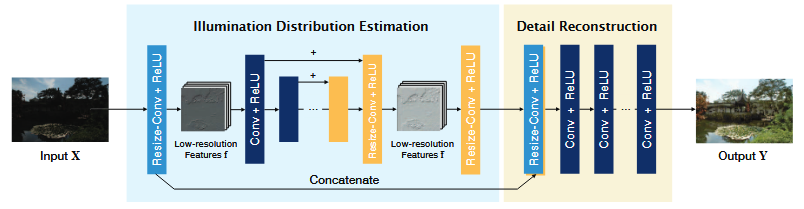
\includegraphics[width=0.8\columnwidth]{GLADNet}
	
	\begin{subfigure}{0.19\textwidth}
		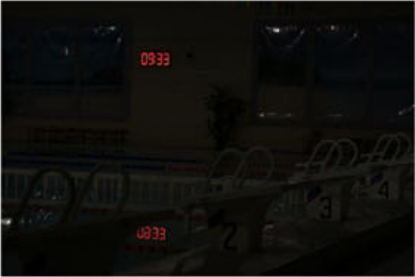
\includegraphics[width=\linewidth]{picture/LLIE/Efficent/Input}
		\captionsetup{font=scriptsize}
		\caption{Input}
		\label{fig: Input}
	\end{subfigure}
	\begin{subfigure}{0.19\textwidth}
		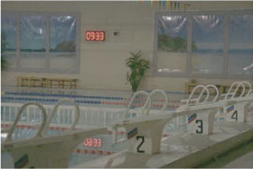
\includegraphics[width=\linewidth]{picture/LLIE/Efficent/LightenNet}
		\captionsetup{font=scriptsize}
		\caption{LightenNet}
		\label{fig: LightenNet}
	\end{subfigure}
	\begin{subfigure}{0.19\textwidth}
		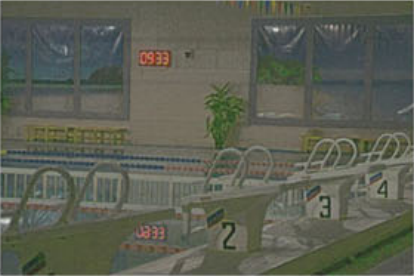
\includegraphics[width=\linewidth]{picture/LLIE/Efficent/LLNet}
		\captionsetup{font=scriptsize}
		\caption{LLNet}
		\label{fig: LLNet}	
	\end{subfigure}
	\begin{subfigure}{0.19\textwidth}
		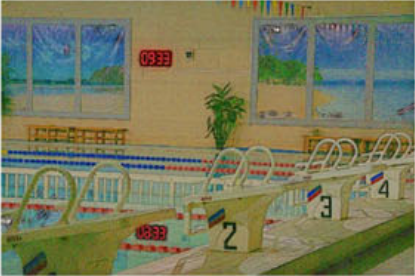
\includegraphics[width=\linewidth]{picture/LLIE/Efficent/RetinexNet}
		\captionsetup{font=scriptsize}
		\caption{RetinexNet}
		\label{fig: RetinexNet}	
	\end{subfigure}
	\begin{subfigure}{0.19\textwidth}
		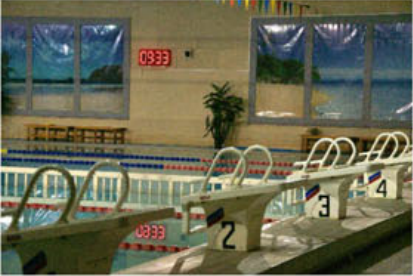
\includegraphics[width=\linewidth]{picture/LLIE/Efficent/KinD}
		\captionsetup{font=scriptsize}
		\caption{KinD}
		\label{fig: KinD}	
	\end{subfigure}\\
	\begin{subfigure}{0.19\textwidth}
		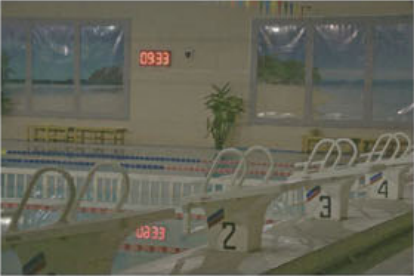
\includegraphics[width=\linewidth]{picture/LLIE/Efficent/MBLLEN}
		\captionsetup{font=scriptsize}
		\caption{MBLLEN}
		\label{fig: MBLLEN}	
	\end{subfigure}
	\begin{subfigure}{0.19\textwidth}
		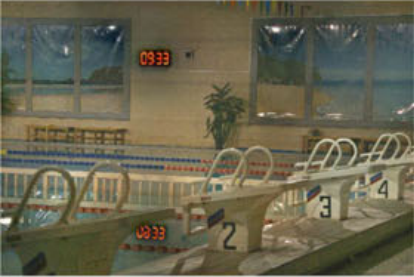
\includegraphics[width=\linewidth]{picture/LLIE/Efficent/EnlightenGAN}
		\captionsetup{font=scriptsize}
		\caption{EnlightenGAN}
		\label{fig: EnlightenGAN}	
	\end{subfigure}
	\begin{subfigure}{0.19\textwidth}
		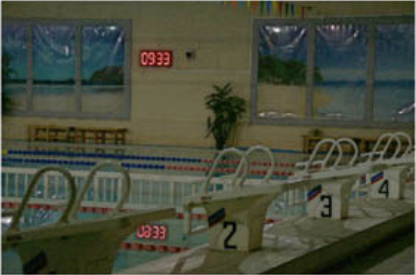
\includegraphics[width=\linewidth]{picture/LLIE/Efficent/Zero-DCE}
		\captionsetup{font=scriptsize}
		\caption{Zero-DCE}
		\label{fig: Zero-DCE}	
	\end{subfigure}
	\begin{subfigure}{0.19\textwidth}
		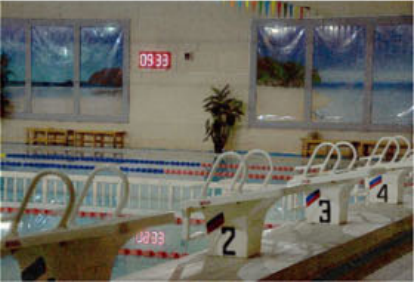
\includegraphics[width=\linewidth]{picture/LLIE/Efficent/Ours}
		\captionsetup{font=scriptsize}
		\caption{Ours}
		\label{fig: Ours}	
	\end{subfigure}
	\begin{subfigure}{0.19\textwidth}
		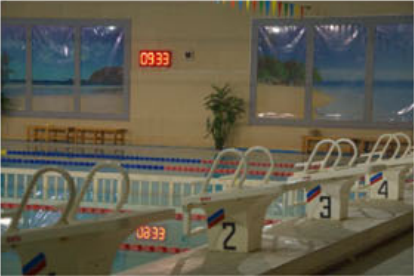
\includegraphics[width=\linewidth]{picture/LLIE/Efficent/GT}
		\captionsetup{font=scriptsize}
		\caption{GT}
		\label{fig: GT}	
	\end{subfigure}
	%\captionsetup{font=scriptsize}
	\caption{
		\label{fig: LOL}
		不同方法在LOL测试数据集上的视觉表现。
	}
\end{figure}

图\ref{fig: LOL}展示了各种方法在LOL测试数据集上的图像增强效果,其中GT表示真实图片。与Zero-DCE、LLNet和MBLLEN相比,RetinexNet呈现出颜色饱和度更强的增强效果,而Zero-DCE、LLNet和MBLLEN的结果在视觉上偏暗。EnlightenGAN在增强的图像中显示出明显的灰色伪影,表明其对噪声较为敏感。尽管我们的方法相对真实值而言稍显偏亮,但在LOL数据集上表现出优于对比方法的效果。

\subsection{消融实验}

我们采用PSNR、SSIM和NIQE指标,对SCConv模块、Transformer分支以及基于不同尺寸的预训练视觉变换器模型的有效性进行评估。我们设定去除SCConv模块的CNN分支作为基线网络。如表\ref{tab: Ablation Study}所示,引入Transformer分支并增加输入到Transformer分支的特征图尺寸,相较于基线,模型性能得到了显著改善。

\begin{table}[!htbp]
	\centering
	\tiny
	\resizebox{\textwidth}{!}{ %按照宽度调整调整表格大小
		\begin{tabular}{c|c|c|c|c|c|c}
			
			\hline
			
			\textbf{基线模型} & \textbf{SCConv} & \textbf{Transformer分支} & \textbf{Transformer预训练权重尺寸}  & \textbf{PSNR↑} & \textbf{SSIM↑} & \textbf{NIQE↓} \\

			\hline
			
			\checkmark &            &            &                  & 18.222 & 0.642 & 7.213 \\
			\checkmark & \checkmark &            &                  & 18.231 & 0.523 & 5.231 \\
			\checkmark & \checkmark & \checkmark & $224 \times 224$ & 21.643 & 0.815 & 4.552 \\
			\checkmark & \checkmark & \checkmark & $384 \times 384$ & \textbf{22.780} & \textbf{0.823} & \textbf{4.473} \\

			\hline			
		\end{tabular}
	}
	%\captionsetup{font=scriptsize} %设置标题字体与表格字体一致
	\caption{
		\label{tab: Ablation Study}
		Transformer分支和Transformer预训练权重尺寸和SCConv对模型的影响。
	} 
\end{table}

\section{总结}

本研究提出了PACUT算法,用于有效增强弱光图像。该算法采用并行结构,融合了CNN分支和Transformer分支,以有效提取特征图的长距离和短距离特征。具体而言,CNN分支采用改进的U型网络架构,包括编码器子网络和解码器子网络。编码器子网络由多层卷积网络组成,每层集成了空间注意力机制和通道注意力机制。Transformer分支以视觉变换器为核心,利用其自注意力机制提取图像的全局特征,为CNN分支提供补充和增强。这些设计不仅增强了弱光图像的信息,还有效避免了增强过度和不足。然而,模型可能过于偏向短距离特征,结构上CNN分支较为冗余,而Transformer分支相对瘦小。未来的工作中,将深入探索Transformer编码器和CNN结构的并行架构,借鉴Conformer模型中多个Transformer编码器块以捕获更多长距离特征。

此外,现有研究主要关注亮度细化,却忽视了色度的重要性。同时,这些方法在优化弱光图像与真实图像之间的外观距离时,往往忽略了物体边缘的模糊问题,可能导致图像细节的损失,进而影响结构相似性指数(SSIM)。未来的工作中,将结合图像的边缘信息,以更好地指导弱光图像增强。


	
\renewcommand{\refname}{\zihao{-4}参考文献}
	
	%	\begin{thebibliography}{00}
		
		%		\bibitem{b1}\label{cite:b1}
		%		W. Wang, C. Wei, W. Yang and J. Liu, "GLADNet: Low-Light Enhancement Network with Global Awareness," 2018 13th IEEE International Conference on Automatic Face \& Gesture Recognition (FG 2018), Xi'an, China, 2018, pp. 751-755, DOI: 10.1109/FG.2018.00118.
		
		%		\bibitem{b2}\label{cite:b2}
		%		A.\ Mahajan, K.\ Somaraj and M. Sameer, "Adopting Artificial Intelligence Powered ConvNet To Detect Epileptic Seizures," 2020 IEEE-EMBS Conference on Biomedical Engineering and Sciences (IECBES), Langkawi Island, Malaysia, 2021, pp. 427-432, DOI: 10.1109/IECBES48179.2021.9398832.
		
		%		\bibitem{Cyr}
		%		N.\ Cyr, M.\ T$\hat{e}$tu, and M.\ Breton,
		% "All-optical microwave frequency standard: a proposal,"
		%		IEEE Trans.\ Instrum.\ Meas.\ \textbf{42}, 640 (1993).
		
		
		
		%	\end{thebibliography}
	
{\zihao{-5}\bibliographystyle{unsrt}
\bibliography{reference}}
	
	
\end{document}